\documentclass{article}
\usepackage{graphicx} % Required for inserting images

\title{Zadanie na Warsztat programisty}
\author{Łukasz Kulpaczyński}
\date{January 2024}

\begin{document}

\maketitle % Stworzenie strony tytułowej

\begin{abstract}
Streszczenie: lorem ipsum.
\end{abstract}

\tableofcontents % Spis treści
\newpage

\section{Wprowadzenie}
Lorem ipsum \cite{hawking1974} dolor sit amet, consectetur adipiscing elit. Vivamus luctus congue tellus et lobortis. Donec sed ipsum purus. Ut nunc risus, congue et urna non, vulputate eleifend urna. Praesent egestas ipsum eu orci tincidunt laoreet. Vestibulum quis viverra sem, \cite{shannon1948} vel fermentum felis. Phasellus nulla felis, sollicitudin vitae orci et, imperdiet iaculis mi. Cras sit amet elementum nunc. Duis enim mi, bibendum eu imperdiet a, convallis vel est. Etiam facilisis tristique sem, sed ullamcorper velit ultricies at.
\subsection{Podsekcja}
Rozdział 1.

\section{Główna część pracy}
Suspendisse potenti.\cite{knuth1984} Suspendisse metus velit, tincidunt in tincidunt non, interdum non justo. Sed sit amet est nec enim viverra aliquet. Nullam interdum lectus purus, ut gravida augue maximus et. In maximus auctor nisl pulvinar auctor. Integer varius augue ac turpis faucibus, at aliquet justo placerat. Integer efficitur sem lectus, a congue tortor dignissim eu. Suspendisse vel velit at mauris pulvinar laoreet consectetur in lacus. Pellentesque congue neque turpis, non pharetra mauris ultrices a.\cite{mccarthy1960}

\subsection{Podsekcja}
Donec pulvinar dolor eu felis mollis placerat. Aliquam vestibulum sed risus ultricies lacinia. In elit leo, bibendum vel mi sed, commodo auctor nisi. Duis in condimentum mi. Donec tempus porta turpis vel gravida. Donec sodales sem id turpis dictum, quis lobortis elit pulvinar. \cite{turing1936}Maecenas odio sapien, maximus ut lorem id, porta euismod ligula. Maecenas bibendum posuere metus sed finibus. Suspendisse massa sem, tristique nec sem sed, porta accumsan elit. Ut enim dui, vulputate vitae odio molestie, sagittis pretium risus. Vivamus non cursus diam.

\subsubsection{Podpodsekcja}
Maecenas rutrum tortor ac lacus laoreet fermentum. Duis eget purus sed diam mollis dignissim eget eget quam. Sed nec est placerat, bibendum nibh sed, ultricies ipsum. Morbi pharetra nisi ut lectus dapibus posuere. Etiam malesuada, odio at blandit lacinia, magna nunc tincidunt tortor \cite{codd1970}, in porta nibh leo id augue. Integer quis quam eget est fringilla mattis. Cras facilisis erat nec ullamcorper eleifend. Vestibulum lorem eros, posuere eget enim eget, blandit gravida lorem. Phasellus convallis finibus tellus, vitae fringilla metus laoreet ultrices. Fusce eget fringilla tellus, a sodales felis. Quisque scelerisque sodales erat, vel dictum ex vehicula sed.

% Przykład pogrubienia i podkreślenia
\textbf{Pogrubiony tekst}, \underline{podkreślony tekst}.

% Przykład trybu matematycznego
Równania matematyczne: $E=mc^2$.

\begin{equation}
    P(X=k) = p^k (1-p)^{1-k}
\end{equation}
% Przykład wstawienia grafiki
\begin{figure}[h]
\centering
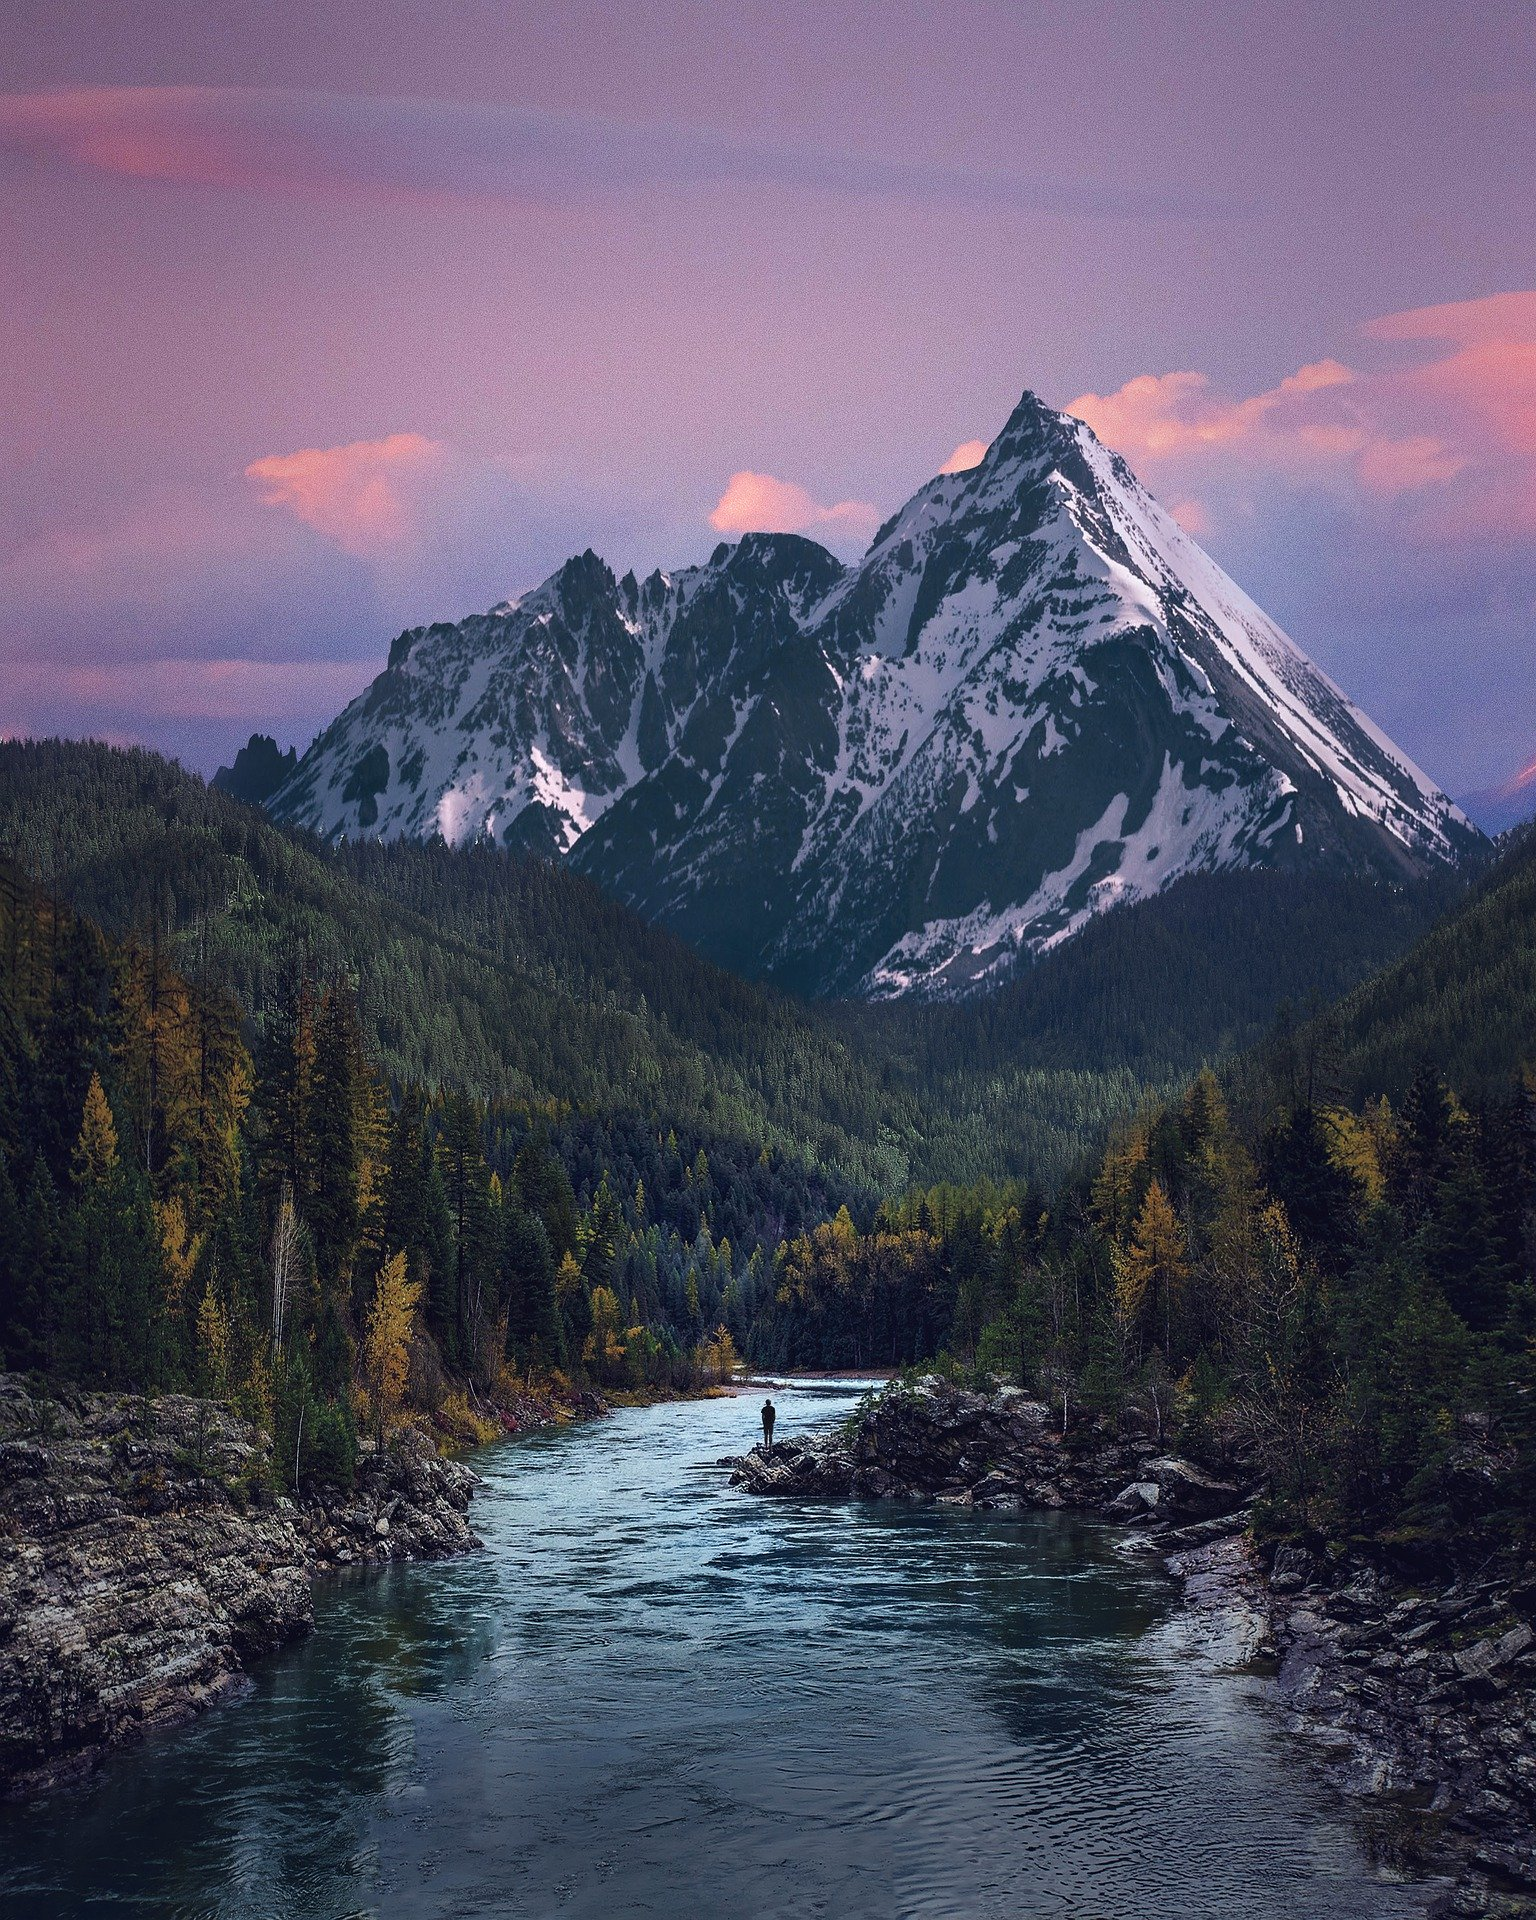
\includegraphics[width=0.5\textwidth]{valley.jpg}
\caption{Opis grafiki}
\label{fig:grafika1}
\end{figure}

\begin{figure}[h]
\centering
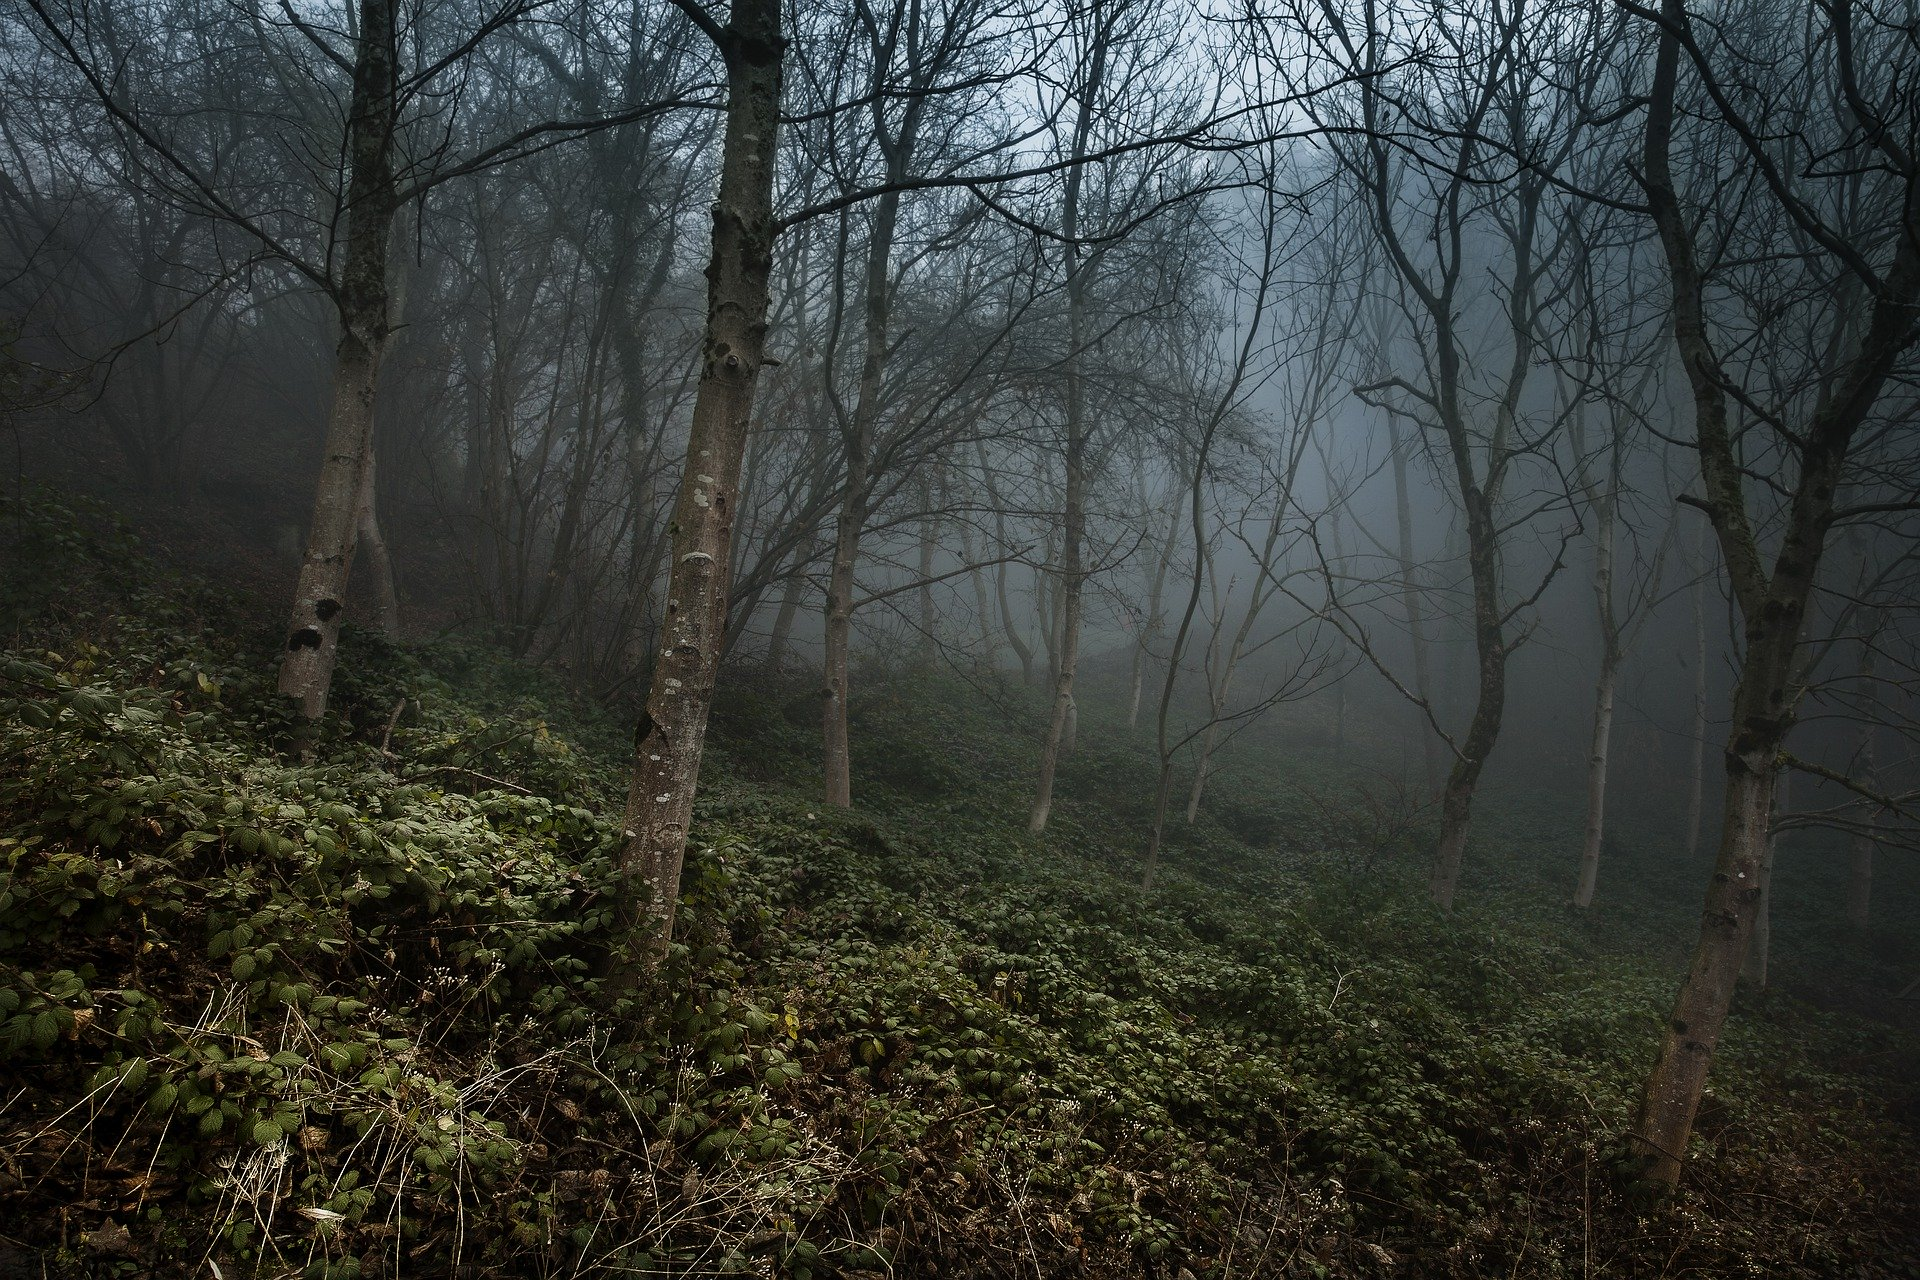
\includegraphics[width=0.5\textwidth]{foggy.jpg}
\caption{Opis drugiej grafiki}
\label{fig:grafika2}
\end{figure}

% Przykład wstawienia tabeli
\begin{table}[h]
\centering
\begin{tabular}{|c|c|}
\hline
Kolumna 1 & Kolumna 2 \\
\hline
Dane 1 & Dane 2 \\
\hline
\end{tabular}
\caption{Opis tabeli}
\label{tab:tabela1}
\end{table}

% Przykład odwołań do grafik i tabel
Jak pokazano na Rysunku \ref{fig:grafika1} i w Tabeli \ref{tab:tabela1} Integer quis quam eget est fringilla mattis. Cras facilisis erat nec ullamcorper eleifend. Vestibulum lorem eros, posuere eget enim eget, blandit gravida lorem. Phasellus convallis finibus tellus, vitae fringilla metus laoreet ultrices. Fusce eget fringilla tellus, a sodales felis. Quisque scelerisque sodales erat, vel dictum ex vehicula sed.

\newpage








% Bibliografia
\bibliographystyle{plain}
\bibliography{data}

\end{document}
